\documentclass[12pt]{report}
\usepackage{graphicx}
\usepackage[utf8]{inputenc}
\usepackage{alphabeta}
\usepackage{hyperref}

 
\graphicspath{ {images/} }

\title{
    {Κατασκευή Έξυπνης, Τηλεχειριζόμενης Κλειδαριάς Θυροτηλεφώνου με χρήση Τεχνολογιών Αιχμής }\\
    {\large Πανεπιστήμιο Πειραιώς}
}
\author{Κυριάκος Δ. Γιαννάκης}
\date{Day Τεστ Year}

\begin{document}
    \maketitle
    
    \begin{abstract}
        TODO
    \end{abstract}
    
    \tableofcontents
    
    \chapter{Εισαγωγή}
    Στον σημερινό κόσμο, οι τεχνολογικές μας ανάγκες γίνονται ολοένα και πιο πολύπλοκες. Κάθε μέρα βγαίνουν στην επιφάνεια νέες τεχνολογικές διευκολύνσεις για τον άνθρωπο, σκοπός των οποίων είναι να κάνουν την διαβίωσή του πιο "έξυπνη", δίνοντάς του τον μέγιστο έλεγχο σε κάθε σημείο της ζωής του. Με την άνθιση του internet of things, γίνεται εύκολη η διασύνδεση πολλών συσκευών (από την μικρότερη ως την μεγαλύτερη), με σκοπό τον έλεγχό τους απομακρυσμένα.

\textbf{Σκοπός της παρούσας πτυχιακής εργασίας είναι να περιγράψει την πλήρη διαδικασία του σχεδιασμού και υλοποίησης ενός συστήματος ελέγχου κλειδαριάς σπιτιού/γραφείου, γνωστό ως PiLock.}

Η εφαρμογή υλοποιήθηκε, στο μεγαλύτερο μέρος της, χρησιμοποιόντας λογισμικό τελευταίας τεχνολογίας, πράγμα που μας εγγυάται την μέγιστη ευελιξία όσων αφορά την ανάπτυξη, πράγμα που ισοδυναμεί με μέγιστη ταχύτητα ανάπτυξης και αυξημένη ασφάλεια. %Αξίζει σε αυτό το σημείο να αναφέρουμε οτι δεν πρέπει να μπερδεύουμε το λογισμικό τελευταίας τεχνολογίας με το Bleeding Edge Software (Λογισμικό τεχνολογίας αιχμής).

\section{Internet of Things}
	Ο όρος "Internet of Things"(IoT) χρησιμοποιήθηκε πρώτη φορά από τον Kevin Ashton το 1999 σε μία παρουσίασή του στην Procter \& Gamble (P\&G) \cite{iotterm}. Ο όρος επινοήθηκε προκειμένου να μπορεί να τονιστεί η δύναμη της (τότε) δημοφιλούς ιδέας της χρήσης της τεχνολογίας RFID σε συστήματα εφοδιαστικών αλυσίδων εταιριών για παρακολούθηση εμπορευμάτων. Πλέον, ο όρος Internet of Things χρησιμοποιείται προκειμένου να χαρακτηριστούν συσκευές (μικρές ή μεγάλες) με δυνατότητα σύνδεσης στο Internet. Κάποια παραδείγματα είναι τα αυτοκίνητα με ενσωματομένους αισθητήρες, τα έξυπνα σπίτια (τα οποία αποτελούνται από μια πληθώρα έξυπνων συσκευών), καθώς επίσης και συγκεκριμένες συσκευές παρακολούθησης υγείας (όπως πχ. συσκευές παρακολούθησης καρδιακού ρυθμού) με δυνατότητα σύνδεσης στο διαδίκτυο.

	Οι δυνατότητες που έχουν οι συγκεκριμένες συσκευές τις καθιστούν ικανές για σύνδεση στο internet, και κατ'επέκταση, αυξάνουν σημαντικά τις λειτουργίες τους, προσδίδοντας μεγαλύτερο έλεγχο στον χρήστη. %Check it...

\section{Αυτοματισμοί Σπιτιού - Home Automation}
	Μία από τις πιο σημαντικές υποκατηγορίες των συσκευών Internet of Things είναι οι \textbf{συσκευές αυτοματισμού σπιτιών (Home Automation Devices, Domotics \cite{domotics} )}. Οι συσκευές αυτές δίνουν στον χρήστη τους την δυνατότητα να διαχειριστεί διάφορες συσκευές του σπιτιού/γραφείου του. Οι συσκευές αυτές μπορεί να είναι συσκευές κλιματισμού, φωτισμός, συστήματα διασκέδασης (Home Theaters, Music Stereos, κτλ...), καθώς επίσης και συστήματα συναγερμού ή και διαχείρησης πρόσβασης. Το PiLock ανήκει στην τελευταία αυτή κατηγορία.

	Συνήθως, οι συσκευές αυτές συνδέονται σε ένα κεντρικό κόμβο (Hub) προκειμένου να ελέγχονται όλες από ένα μοναδικό σημείο. Η δυνατότητα αυτή μπορεί να προστεθεί σε μία επόμενη έκδοση του PiLock (βλ. μελλοντικά σχέδια). Την παρούσα χρονική στιγμή, δεν υπάρχει αυτή η δυνατότητα.

\section{Σκοπός του PiLock}
	Το PiLock ανήκει στην κατηγορία συσκευών \textbf{"έξυπνου σπιτιού" (Smart Home)}. Σκοπός του είναι να παρέχει στον χρήστη την δυνατότητα να ξεκλειδώνει εύκολα την εξώπορτα/πόρτα του σπιτιού/γραφείου του, μέσω του SmartPhone ή του SmartWatch του, όλα αυτά χρησιμοποιόντας το ασφαλέστερο δυνατόν περιβάλλον, προκειμένου να αποφευχθεί εισβολή τρίτων.

	Μέσω του \textbf{PiLock Administration Control Panel (PiLock AdminCP)}, δίνουμε στον διαχειριστή του συστήματος ένα εύχρηστο περιβάλλον διαχείρησης από το οποίο μπορεί εύκολα και γρήγορα να διαχειρίζεται το PiLock. Δίνεται δυνατότητα διαχείρησης των \textbf{εξουσιοδοτημένων χρηστών (χρήστες που μπορούν να ξεκλειδώσουν την πόρτα μέσω του PiLock)}, δυνατότητα λήψης ζωτικής σημασίας πληροφοριών για το σύστημα, καθώς επίσης και της δυνατότητας ξεκλειδώματος της πόρτας απευθείας μέσω του πίνακα διαχείρησης, χωρίς να χρειάζεται να γίνει χρήση της εφαρμογής (AdminCP Unlock).




    \chapter{Δομή του PiLock}
    To PiLock αποτελείται από 2 κύρια μέρη: Τον εξυπηρετητή (Server) και τον πελάτη (Client).

\section{Σύντομη Περιγραφή Λογισμικού Εξυπηρετητή - PiLock Server}
	Ο εξυπηρετητής αποτελείται από το Hardware που χρειάζεται προκειμένου να λειτουργήσει το PiLock, καθώς επίσης και το αντίστοιχο λογισμικό υπεύθυνο για την διαχείρηση της κλειδαριάς, από όλες τις απόψεις. Πιο συγκεκριμένα, το λογισμικό είναι υπεύθυνο για:
	\begin{itemize}
		\item Την διαχείριση του Hardware υπεύθυνου για την λειτουργία του μηχανισμού ξεκλειδώματος.
		\item Την αυθεντικοποίηση των ήδη υπάρχοντων χρηστών.
		\item Την δημιουργία νέων χρηστών, ικανών για αυθεντικοποίηση (εξουσιοδοτημένοι χρήστες).
		\item Την τήρηση ιστορικού αυθεντικοποιήσεων (επιτυχών ή μή).
	\end{itemize}
	Το λογισμικό του εξυπηρετητή αναλύεται πλήρως στην αντίστοιχη ενότητα. %TODO FIX IT

\section{Σύντομη Περιγραφή Λογισμικού Πελάτη - PiLock Client}
	Η πλευρά του πελάτη αποτελείται από την εφαρμογή του PiLock, σχεδιασμένη για κινητά που τρέχουν Android, καθώς επίσης και από την εφαρμογή σχεδιασμένη για Android Wear Smartwatches.

	Πιο συγκεκριμένα, οι εφαρμογές στο πεδίο του πελάτη είναι υπεύθυνες για:

	\begin{itemize}
		\item Σύνδεση στην πλατφόρμα του PiLock\textsuperscript{*}.
		\item Αποστολή αιτημάτων ξεκλειδώματος.
		\item Αποστολή αιτημάτων αλλαγής PIN\textsuperscript{*}.
	\end{itemize}
	{\footnotesize Οι δυνατότητες που είναι σημειωμένες με τον αστερίσκο (*) είναι διαθέσιμες αποκλειστικά στην εφαρμογή για κινητά (mobile app) και όχι στην εφαρμογή για Android Wear.}

\section{Υλικό - Hardware}
	Όπως αναφέραμε και στην εισαγωγή, ένας εκ των στόχων από τις πρώτες μέρες του σχεδιασμού του PiLock ήταν να υλοποιηθεί το Project με όσο το δυνατόν λιγότερο κόστος. Προκειμένου αυτό να είναι εφικτό, χρησιμοποιήσαμε υλικό εύκολα προσκομίσιμο και, όπου ήταν δυνατόν, Open Source Hardware.

	\subsection{Raspberry Pi Zero W}
		"Εγκέφαλος" όλης της κατασκευής είναι το Raspberry Pi Zero W (RPi Zero W), ένας υπολογιστής μοναδικής πλακέτας (Single Board). Σχεδιάζεται από το Raspberry Pi Foundation στην Αγγλία και η κυκλοφορία του ξεκίνησε τον Φεβρουάριο του 2017. Σκοπός του RPi Zero W είναι να συμπληρώσει το προηγούμενο μοντέλο, το Raspberry Pi Zero, φέρνοντας δυνατότητες συνδεσιμότητας WiFi 802.11n και BlueTooth 4.0 χωρίς Hardware κάποιου τρίτου (μέχρι προτίστως έπρεπε να χρησιμοποιηθεί κάποιο WiFi ή BlueTooth Dongle προκειμένου να υπάρξει αυτή η συνδεσιμότητα) \textsuperscript{\cite{rpizw}}.

		\begin{figure}[h]
			\centering
				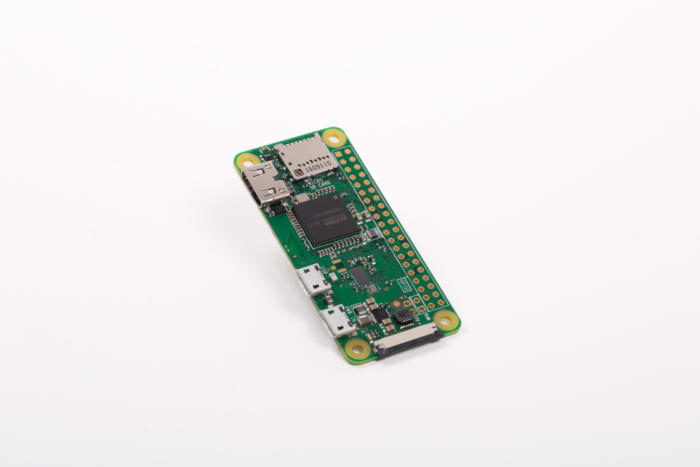
\includegraphics[width=\textwidth,height=\textheight,keepaspectratio]{rpizerow.jpg}
			\caption{Το Raspberry Pi Zero W.}
		\end{figure}

		Στην "καρδιά" του RPi Zero W υπάρχει ένας Broadcom BCM2835, 32-bit επεξεργαστής αρχιτεκτονικής ARMv6, χρονισμένος στο 1Ghz. Για μνήμη τυχαίας προσπέλασης χρησιμοποιούνται 512MB Low Power Double Data Rate 2 (LPDDR2) RAM. Πανω στο RPi Zero W δεν υπάρχει αποθηκευτικός χώρος, οπότε χρησιμοποιείται μια κάρτα MicroSD. 

		Ένα από τα σημαντικότερα σημεία ενός RPi Zero W είναι οι \textbf{δέκτες Εισόδου/Εξόδου Γενικού Σκοπού (GPIO)}. Μέσω αυτών καθίσταται δυνατόν να συνδεθεί το RPi με μια πληθώρα εξωτερικών αισθητήρων, διακοπτών (Relay Modules), πλακετών επέκτασης (γνωστά ως HATs), και εξαρτημάτων και να αντλήσει πληροφορίες ή να τα ελέγξει.

	\subsection{Relay Module}
		\label{sub:relay}
		Προκειμένου να μπορέσει να συνδεθεί το RPi με το ήδη υπάρχον σύστημα ξεκλειδώματος, χρειάζεται ένας ηλεκτρονικά ελεγχόμενος διακόπτης. Θα χρησιμοποιηθεί ένα Relay Module. Τα Relay Modules χρησιμοποιούνται ως διακόπτες προκειμένου να ελέγχονται κυκλώματα μέσω υπολογιστών/μικροελεγκτών, οι οποίοι λειτουργούν μέσω σημάτων μικρής ισχύος\textsuperscript{\cite{relay_purpose}}.

		Τα Relay Modules κυκλοφορούν σε πολλούς τύπους. Οι τρείς κυριότεροι είναι:
		\begin{itemize}
			\item 5V Compatible, Active Low. 
			\item 5V/3.3V Compatible, Active High.
			\item 3.3V Compatible Active High/Low.
		\end{itemize}

		Το Raspberry Pi, εφόσον λειτουργεί σε λογική 3.3V, είναι συμβατό με τους 2 τελευτέους τύπους. Αν θελήσουμε να χρησιμοποιήσουμε ένα Relay Module που να λειτουργεί σε λογική 5V και είναι Active Low, θα χρειαστεί να χρησιμοποιήσουμε ένα Arduino.

		Τα Relay Modules αποτελούνται από ένα Relay τύπου SRD, έναν φωτοσυζευκτή (Optocoupler), ευθύνη του οποίου είναι να απομονώνει το κύκλωμα ωστε να μην επηρρεάσει η υψηλή τάση (σε περίπτωση που χρησιμοποιείται από το σύστημα ξεκλειδώματος του κτηρίου) το υπόλοιπο κύκλωμα, ένα Transistor και μια δίοδο. %TODO Needs citation.

		%TODO Add Figure...

	\subsection{Arduino UNO}
		Το Arduino UNO είναι ένας Ανοικτού-Κώδικα (Open Source) μικροελεγκτής σχεδιασμένος από την \href{https://www.arduino.cc/}{Arduino.cc}. Είναι βασισμένος πάνω στον ATmega328 microcontroller της Atmel. Μπορεί να χρησιμοποιηθεί προκειμένου να χειρίζεται και να αντλεί πληροφορίες από διάφορα εξαρτήματα στον φυσικό κόσμο. Εξαιτίας της μεγάλης ευελιξίας του έχει γίνει μία από τις δημοφιλέστερες επιλογές για κατασκευαστές, οι οποίοι το χρησιμοποιούν για μια τεράστια γκάμα εφαρμογών\textsuperscript{\cite{arduino_definition}}.

		To Arduino UNO μπορεί να χρησιμοποιηθεί σε περίπτωση που δεν χρησιμοποιηθεί κάποιο Relay συμβατό με το Raspberry Pi (βλ. \fullref{sub:relay}), αρκεί να λειτουργεί με λογική 5V.

		Μπορεί, έναντι του Arduino UNO, και προκειμένου να εξοικονομηθεί χώρος, να χρησιμοποιηθεί ένα Arduino Nano, το οποίο έχει όλες τις αναγκαίες λειτουργίες για την λειτουργία του PiLock.

		Ρεύμα για την λειτουργία του Arduino παρέχεται από την θύρα Micro USB του RPi, και μέσω αυτού δίνεται ρεύμα και σε οποιοδήποτε Relay Module συνδεθεί με αυτό. Για να γίνει αποστολή δεδομένων από το RPi στο Arduino χρησιμοποιείται η σειριακή θύρα (Serial Port) του Arduino.

		\begin{figure}[h]
			\centering
				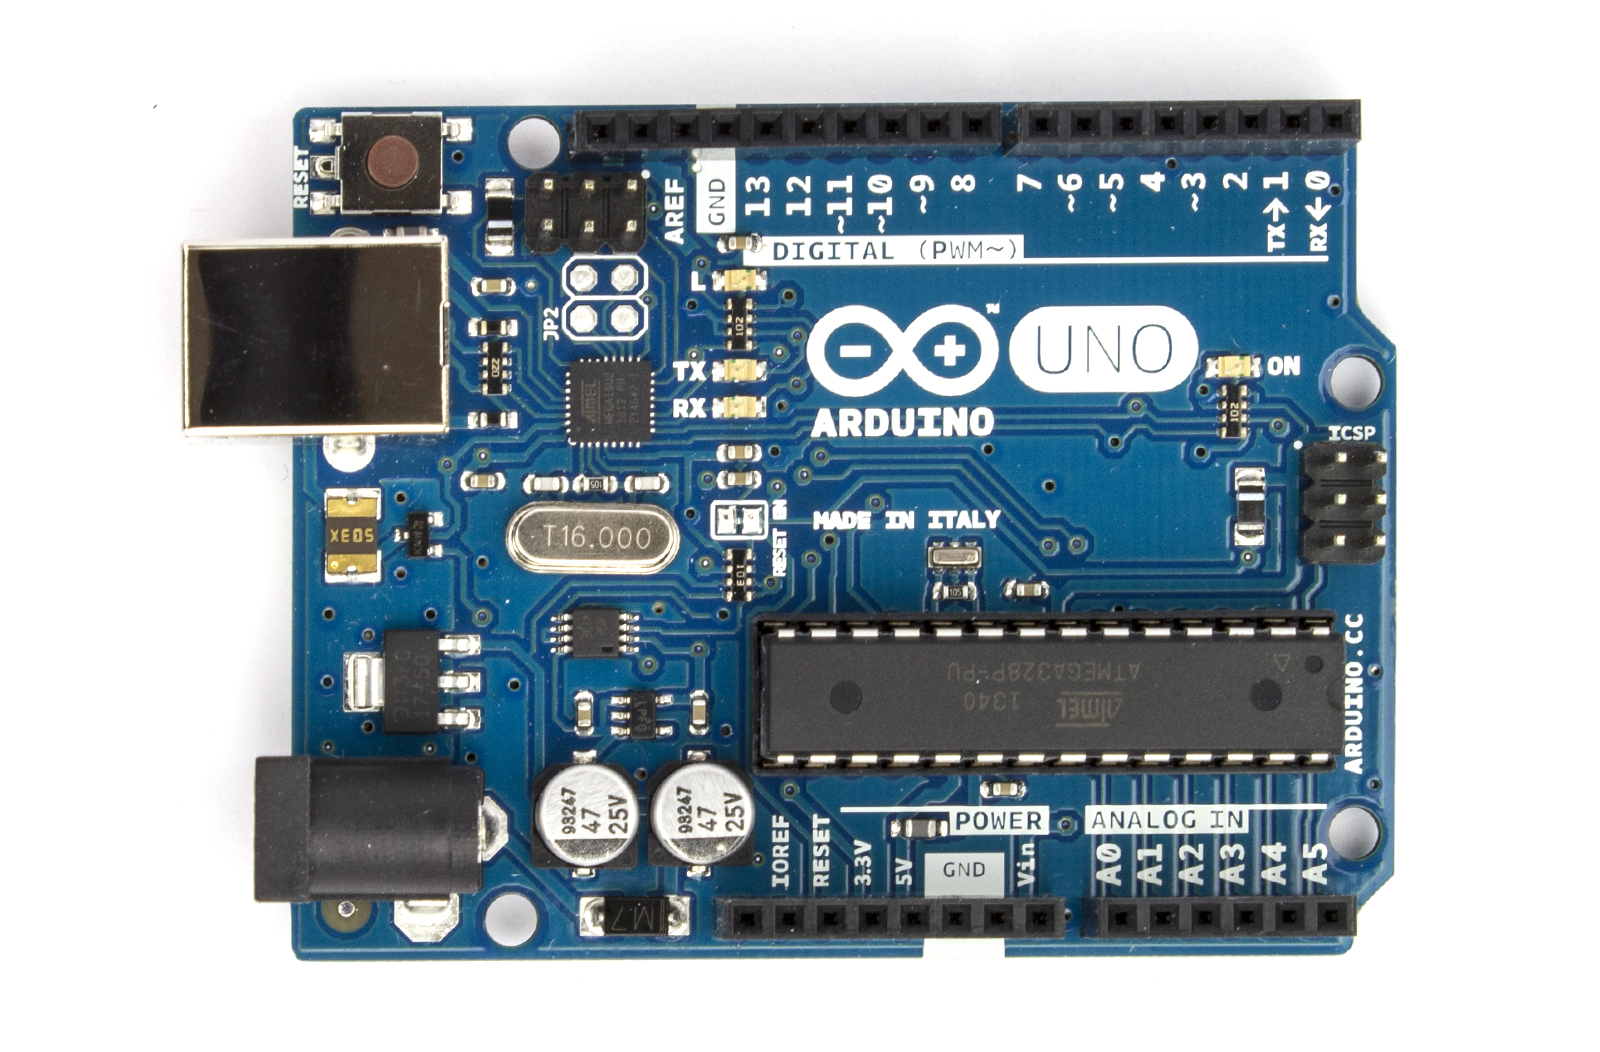
\includegraphics[width=0.5\textwidth,height=0.5\textheight,keepaspectratio]{arduino_uno.jpg}
			\caption{Arduino Uno Rev3, oomlout (2015), Flickr, CC BY-SA 2.0}
		\end{figure}

	\subsection{Λοιπό Hardware}
		Προκειμένου να συναρμολογηθεί η κατασκευή θα χρειαστουν κάποια συγκεκριμένα υλικά.

		\subsubsection{Κουτί Κατασκευής (Project Box)}
			Ανάλογα τον τρόπο σύνδεσης που θα χρησιμοποιηθεί για την σύνδεση του RPi με το Relay Module, και ανάλογα με το αν είναι συμβατό το Relay Module με λογική 3.3V, θα χρειαστεί διαφορετικό μέγεθος κουτιού κατασκευής. 

			\paragraph{Σύνδεση χωρίς χρήση Arduino:}
				Ο προεπιλεγμένος τρόπος σύνδεσης, από την έκδοση 0.3.1 και μετά είναι χωρίς την χρήση Arduino. Έπειτα από μετρήσεις βρέθηκε οτι το κατάλληλο κουτί κατασκευής έχει διαστάσεις 10cm x 10cm.
			\paragraph{Σύνδεση με Arduino:}
				Εφόσον χρειάζεται να γίνει σύνδεση με Arduino (προκειμένου να μπορεί να λειτουργήσει το Relay Module), έπειτα απο μετρήσεις βρέθηκε οτι το κατάλληλο κουτί κατασκευής έχει διαστάσεις 18cm x 14cm.

		\subsubsection{Καλώδια σύνδεσης}
			Για να συνδεθεί το Relay Module με το RPi (ή το Arduino), θα χρειαστούν κάποια συγκεκριμένα καλώδια σύνδεσης γνωστά ως Jumper Wires. Τα Jumper Wires κάνουν εύκολη την σύνδεση σε διάφορα εξαρτήματα καθώς δεν χρειάζονται συγκόλληση \textsuperscript{\cite{jumper_wires}}.

		 	\paragraph{Σύνδεση χωρίς χρήση Arduino:}
		 		Θα χρειαστούν τουλάχιστον 3 Jumper Wires Female-Male (ή Female-Female, σε περίπτωση χρήσης του Male Header).
		 	\paragraph{Σύνδεση με Arduino:}
		 		Θα χρειαστούν τουλάχιστον 3 Jumer Wires Female-Male, αν χρησιμοποιηθεί Arduino UNO ή 3 τουλάχιστον καλώδια Female-Female, αν χρησιμοποιηθεί Arduino Nano. Επίσης, θα χρειαστεί ένα καλώδιο USB-A to USB-B αν χρησιμοποιηθεί ένα Arduino UNO ή ένα καλώδιο USB-A to Micro USB-B σε περίπτωση χρήσης Arduino Nano.

		 	\begin{figure}[h]
			\centering
				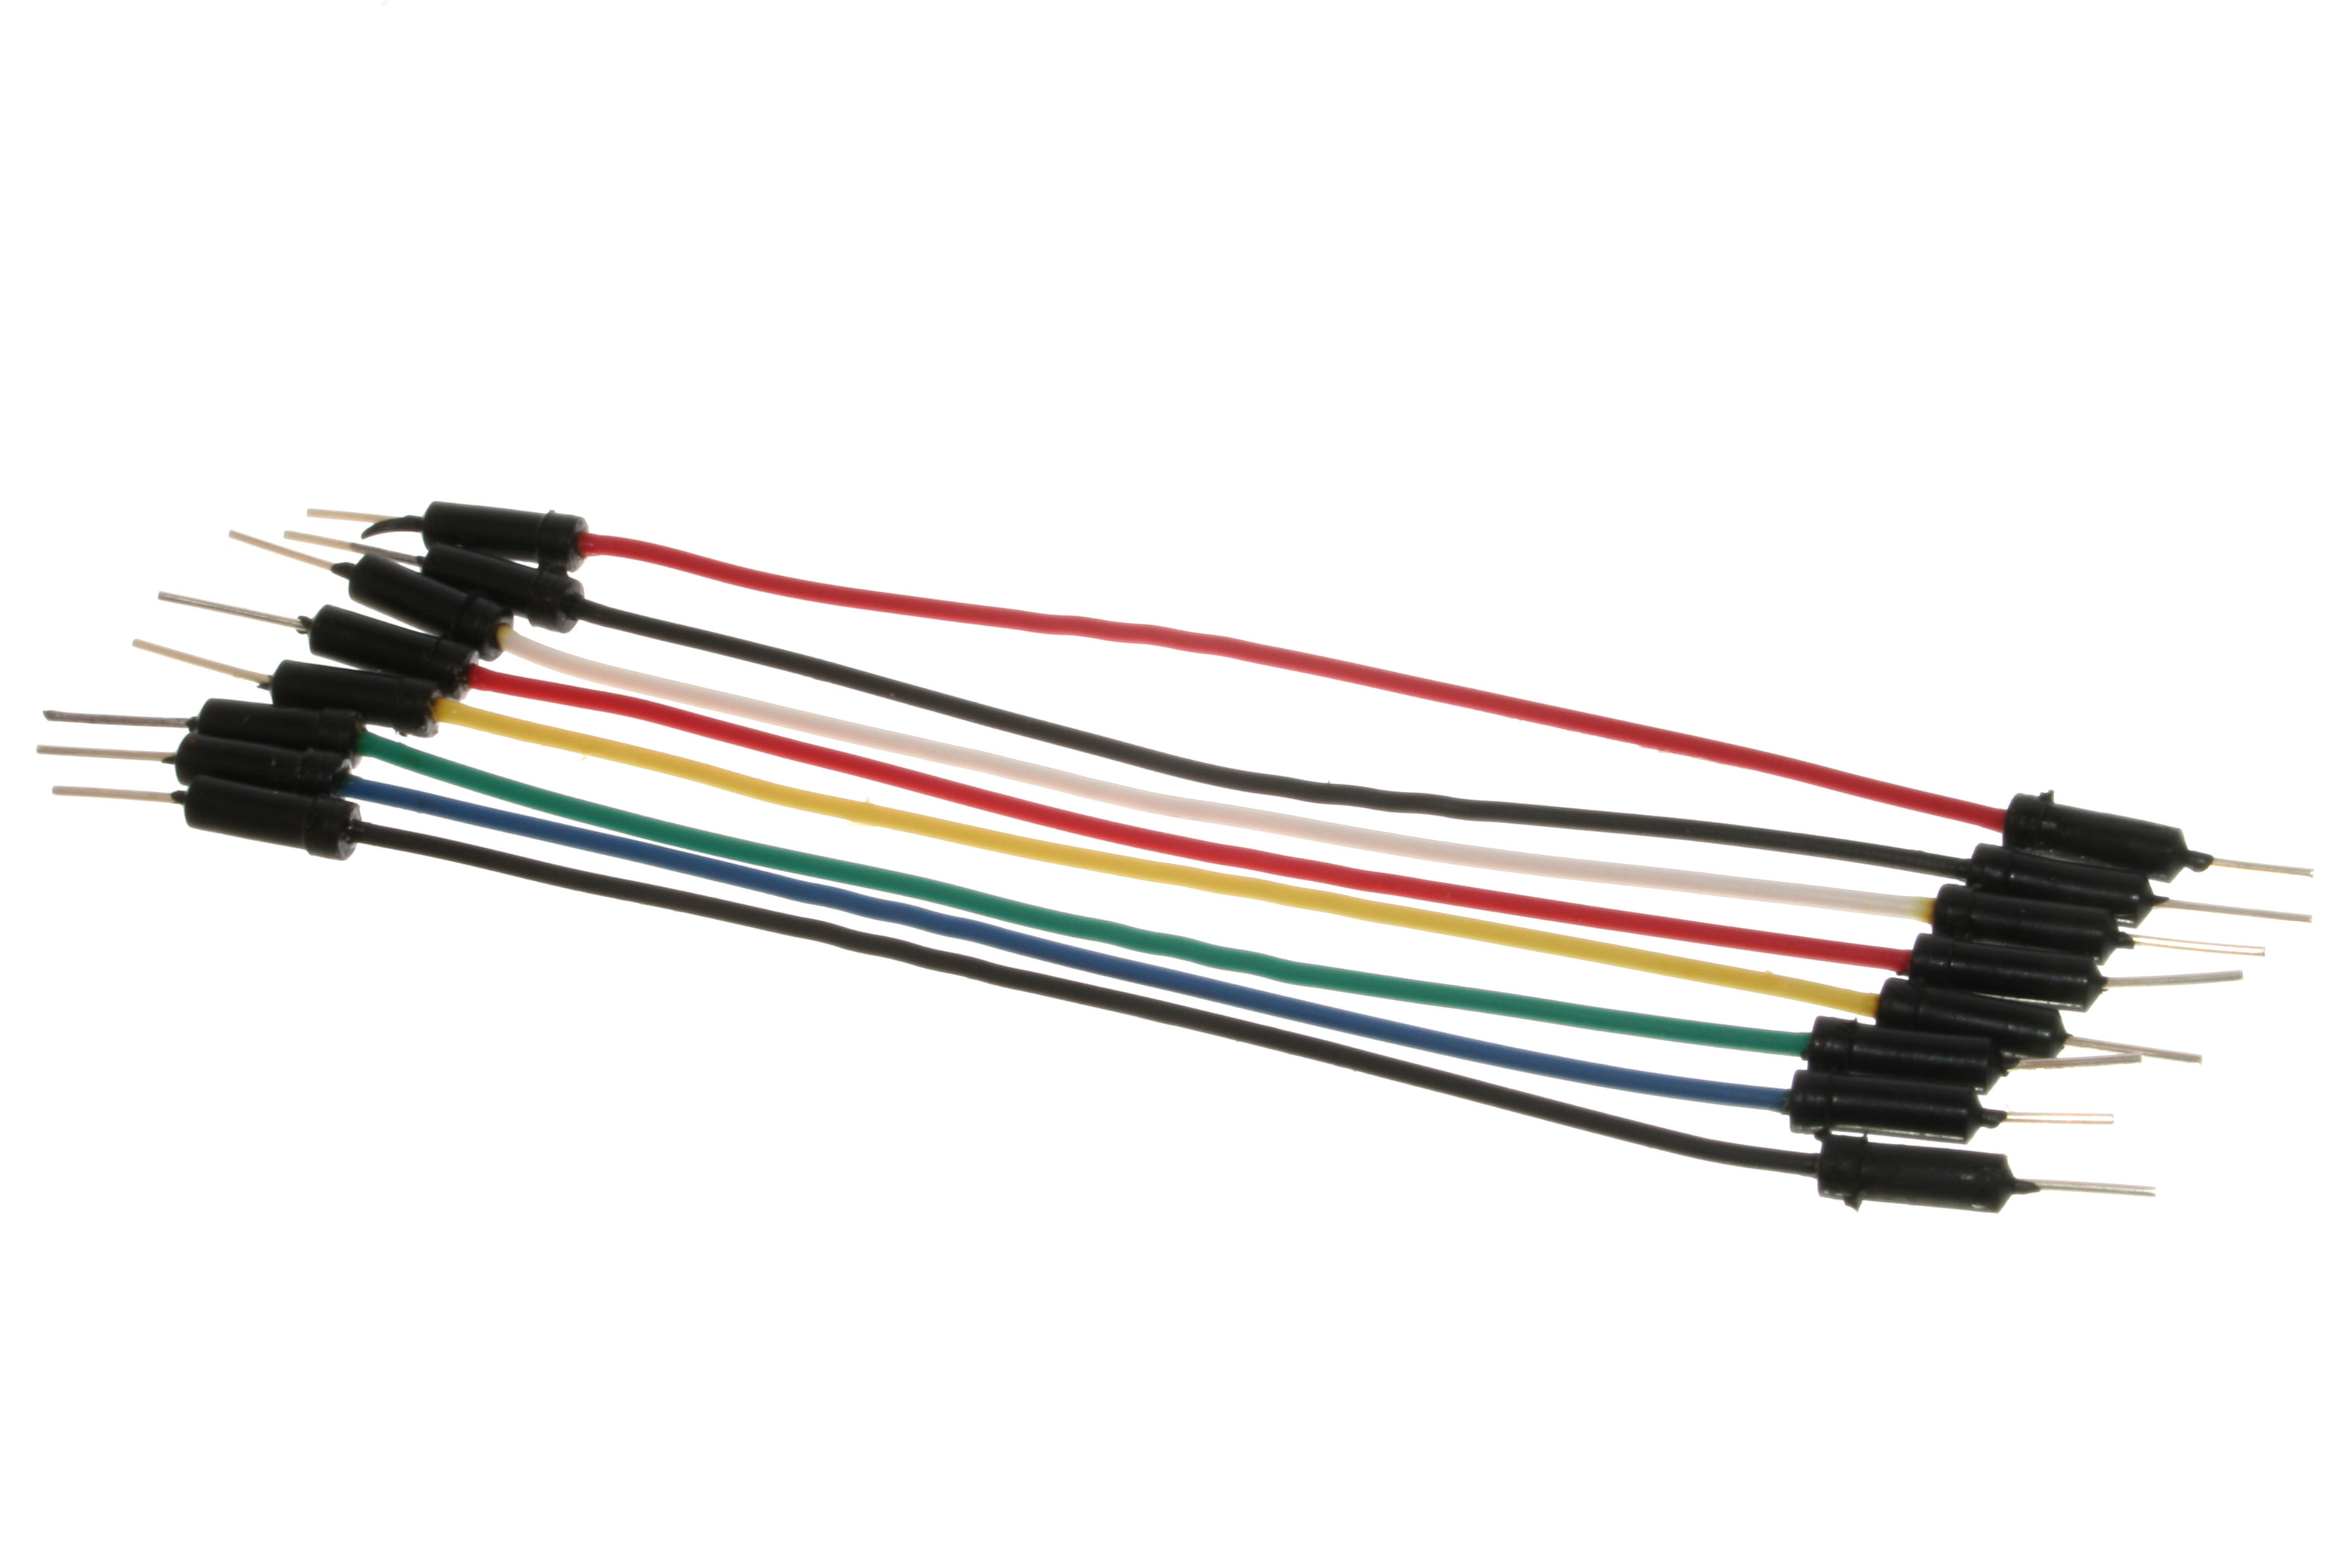
\includegraphics[width=0.5\textwidth,height=0.5\textheight,keepaspectratio]{jumper_wires.jpg}
				\caption{Jumper Wires (Male-Male), oomlout (2009), Flickr, CC BY-SA 2.0}
			\end{figure}

    \begin{thebibliography}{99}

\bibitem{iotterm}
Kevin Ashton (2009), "That 'Internet of Things' thing"\\
\url{http://www.rfidjournal.com/articles/view?4986}

\bibitem{domotics}
Jim Hill (2015), "The smart home: a glossary guide for the perplexed"\\
\url{https://www.t3.com/features/the-smart-home-guide}

\bibitem{rpizw}
Ian Paul (2017), "The \$10 Raspberry Pi Zero W brings Wi-Fi and Bluetooth to the minuscule micro-PC"\\
\url{https://www.pcworld.com/article/3175256/computers/the-10-raspberry-pi-zero-w-brings-wi-fi-and-bluetooth-to-the-minusule-micro-pc.html}

\bibitem{rpizspecs}
Eben Upton (2015), "RASPBERRY PI ZERO: THE \$5 COMPUTER"\\
\url{https://www.raspberrypi.org/blog/raspberry-pi-zero/}

\bibitem{relay_purpose}
Relay, Wikipedia\\
\url{https://en.wikipedia.org/wiki/Relay}

\bibitem{arduino_definition}
Arduino for Beginners, Makerspaces.com\\
\url{https://www.makerspaces.com/arduino-uno-tutorial-beginners/}

\bibitem{jumper_wires}
Jump Wire Structure (2003), Katayama Tatsuo\\
\url{http://www.freepatentsonline.com/6899560.html}

\bibitem{rpi_wifi_headless}
How to connect raspberry pi to WiFi without a monitor (2017), Chetan Kapoor\\
\url{https://installvirtual.com/how-to-connect-raspberry-pi-to-wifi-without-a-monitor/}

\bibitem{raspbian_nov2016_upd}
A security update for Raspbian PIXEL (2016), Simon Long\\ 
\url{https://www.raspberrypi.org/blog/a-security-update-for-raspbian-pixel/}

\bibitem{default_creds}
\url{https://www.raspberrypi.org/documentation/linux/usage/users.md}

\bibitem{secure_passwords}
How to Create a Secure Password You Can Remember Later: 4 Key Methods (2014), Kevan Lee\\
\url{https://open.buffer.com/creating-a-secure-password/}

\bibitem{raspbian_update}
Updating and Upgrading Raspbian
\url{https://www.raspberrypi.org/documentation/raspbian/updating.md}

\bibitem{find_rpi_ip}
\url{https://www.raspberrypi.org/documentation/remote-access/ip-address.md}

\end{thebibliography}
    
\end{document}